\subsection{Phase Space Painting}

Phase space painting is a more sophisticated version of the Orbit Response Matrix method. 
The orbit is changed using a pair of consecutive orbit correctors such that 
position and momentum coordinates of the beam behind the second corrector follow a given ellipse. 
Normally it corresponds to the nominal Twiss parameters at this location or 
to values measured with a quad scan. 
Using these ones maximizes the chances that the beam stays within aperture all along 
the machine as the maximum orbit deviations should follow the nominal $\beta$-function pattern. 
Of course, assuming there is no large optics error. 
Another big advantage is that in this case the reconstructed phase advance can be 
directly compared with the model one. 

This method allows to measure directly phase advance in between BPMs 
independently of their calibration accuracy.  
$\beta$-function is also measured directly as a maximum observed orit amplitude, however, 
its accuracy depends on the BPM calibration.

Each measurement starts with defining 
\begin{enumerate}[nosep]
\item Names of the two corrector devices used to excite the beam
\item Their excitation constants
\item Beam energy $En$
\item Transfer matrix $R_{12}$ and $R_{22}$ components in between the correctors
\item Values of $\alpha$ and $\beta$ Twiss parameters to be painted
\item Area of the ellipse to be painted, i.e. the geometric emittance $\epsilon$
\item Plane (horizontal or vertical)
\item Number of points to paint $N_p$ 
\item Number of beam shots to be recorded for each orbit (usually between 5 and 10)
\end{enumerate}
A set of $\varphi_i$ angles is generated in range between $0$ and $\frac{3\pi}{2}$ 
in step of $\varphi_s = \frac{2\pi}{N_p}$.
Painting larger than $2\pi$ range provides more accurate fits, simply because it increases number of data points.
The spread of the points separated by $2\pi$ also gives a quick visual figure of stability of a particular measurement. 

The order of $\varphi_i$ angles is reshuffled such that 
$\varphi_{2i} - \varphi_{2i-1} = \pi$ and $\varphi_{2(i+1)} - \varphi_{2i} = \pi + \varphi_s$ to make the measurement 
less sensitive to any beam drifts. This reordering is illustrated in Fig.\ref{fig:PhSpEllipseConstr}. 
In this case differences of the consecutively measured orbits enter the analysis instead of 
differences with respect to the reference orbit (the one measured without any corrector magnet excitation). 
Alternatively, the reference orbit would have to be measured after every measurement point what would make 
the measurement twice longer. 

\begin{figure}[!h]
 \begin{center}
  \subfloat[]  %On the plot 16 Dec 2016 14:18
   {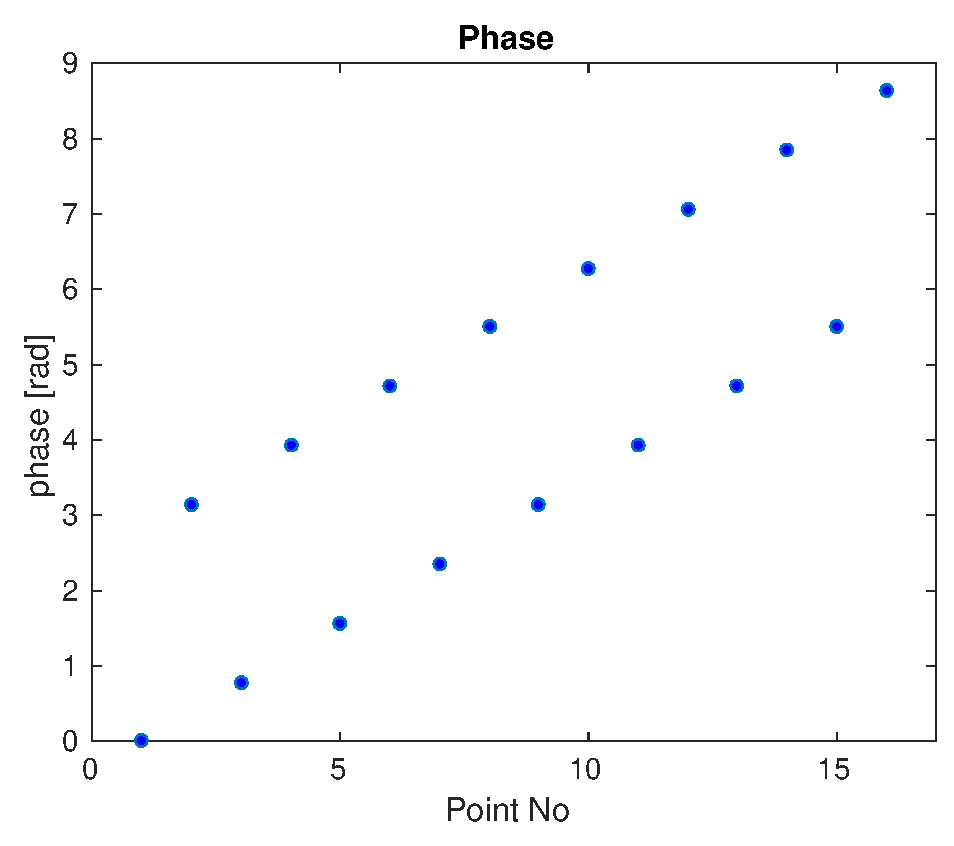
\includegraphics[width=0.45\columnwidth]{PaintedPhases.eps}} 
 \subfloat[]   %On the plot 15 Dec 2016 18:56
   {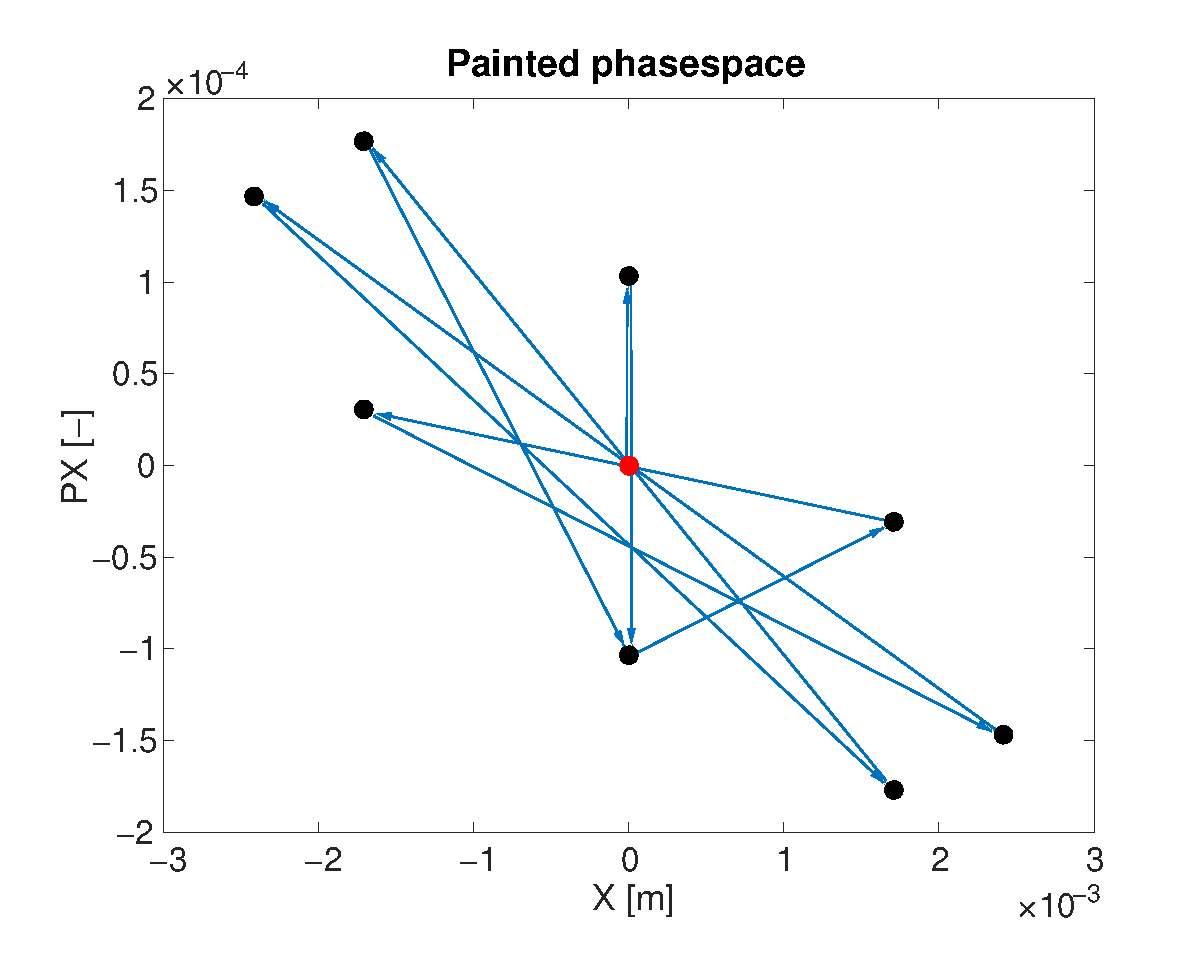
\includegraphics[width=0.51\columnwidth]{PaintedEllipse3.eps}}
 \end{center}
 \caption{Construction of the painted phase space ellipse.}
 \label{fig:PhSpEllipseConstr}
\end{figure}


A phase space ellipse with given $\alpha$, $\beta$ and $\epsilon$ has the following equation
\begin{align}
\begin{split}
   X_{i0}  &=  \sqrt{ \epsilon \beta } *cos(\varphi_i) \\
   XP_{i0} &=  \sqrt{ \frac{\epsilon } {\beta}} (-\alpha cos(\varphi_i)-sin(\varphi_i)) ,
\end{split}
\label{eq302_ellipseEq}
\end{align}
where  $\varphi_i$ is angle of $i_{th}$ point in the normalized coordinates. 
These are produced with the following kicks from orbit correctors 
\begin{align*}
   k_{1i} &=  X_{i0}/R_{12}, \\
   k_{2i} &=  XP_{i0} - k_{1i} \cdot R_{22},
\end{align*}
where $k_{1i}$ and $k_{2i}$ are angles due to upstream and downstream correctors, respectively, 
and $R_{12}$ and $R_{22}$ are components of the transfer matrix in between the two correctors. 
In order to minimize the model dependence of the measurement 
correctors separated only by a drift space were usually selected. 
In this case $R_{22}=1$ and $R_{12}=L_{12}$, where $L_{12}$ is distance in between the correctors. 
Finally, the excitation currents are computed using the particular magnet excitation constant and the beam energy.

Around 10 consecutive beam pulses were recorded for each painted point and 
their averages were used in the analysis. 
%In the first step the orbit differences between the consequtive points were calculated, from which 
Transverse coordinate $X$ was calculated as follows:
\begin{itemize}
 \item for the first point, the simple difference of the excited and the reference obrits, i.e. $X_1 = H_1 - H_0$,
       where $H_0$ and $H_1$ are the measured reference orbit (with no excitation) and the orbit for the first point
 \item for even points, half of difference between the orbit recorded for the given point and the previous one, 
       i.e. $X_{2i} = (H_{2i} - H_{2i-1}) / 2 $
 \item for the remaining odd points $X_{2i+1} = (H_{2i+1} - H_{2i}) - X_{2i}$
\end{itemize}

For each BPM a graph of $X$ in function of the painted phase was constructed.
A function of the form $A_{BPMn} \cdot sin(\varphi + \varphi_{BPMn})$ was fitted,
where $\varphi$ corresponds to abscissa and $A_{BPMn}$ and $\varphi_{BPMn}$ are the fit parameters.
$\varphi_{BPMn}$ measures phase advance between given BPM and the location where the
ellipse is painted, i.e. the downstream orbit corrector.
$A_{BPMn}$ measures size of the ellispe and if the BPM is well callibrated
\begin{equation}
\beta_{BPMn} = A^2_{BPMn}/\epsilon.
\label{eq:betaampl}
\end{equation}

Naturally, for the highest signal to noise ratio an ellipse with the largest area that 
can be transported without losses to the end of the section under study is searched.
In order to verify the procedure it was tested on a long drift line 
with multiple BPMs by depowering all the quadrupoles.
The observed discrepancy in phase advance allowed to correct the eventual errors in 
the excitations constants of the corrector magnets.

\begin{figure}[!h]
 \centering
  \subfloat[]  %On the plot 16 Dec 2016 14:18
   {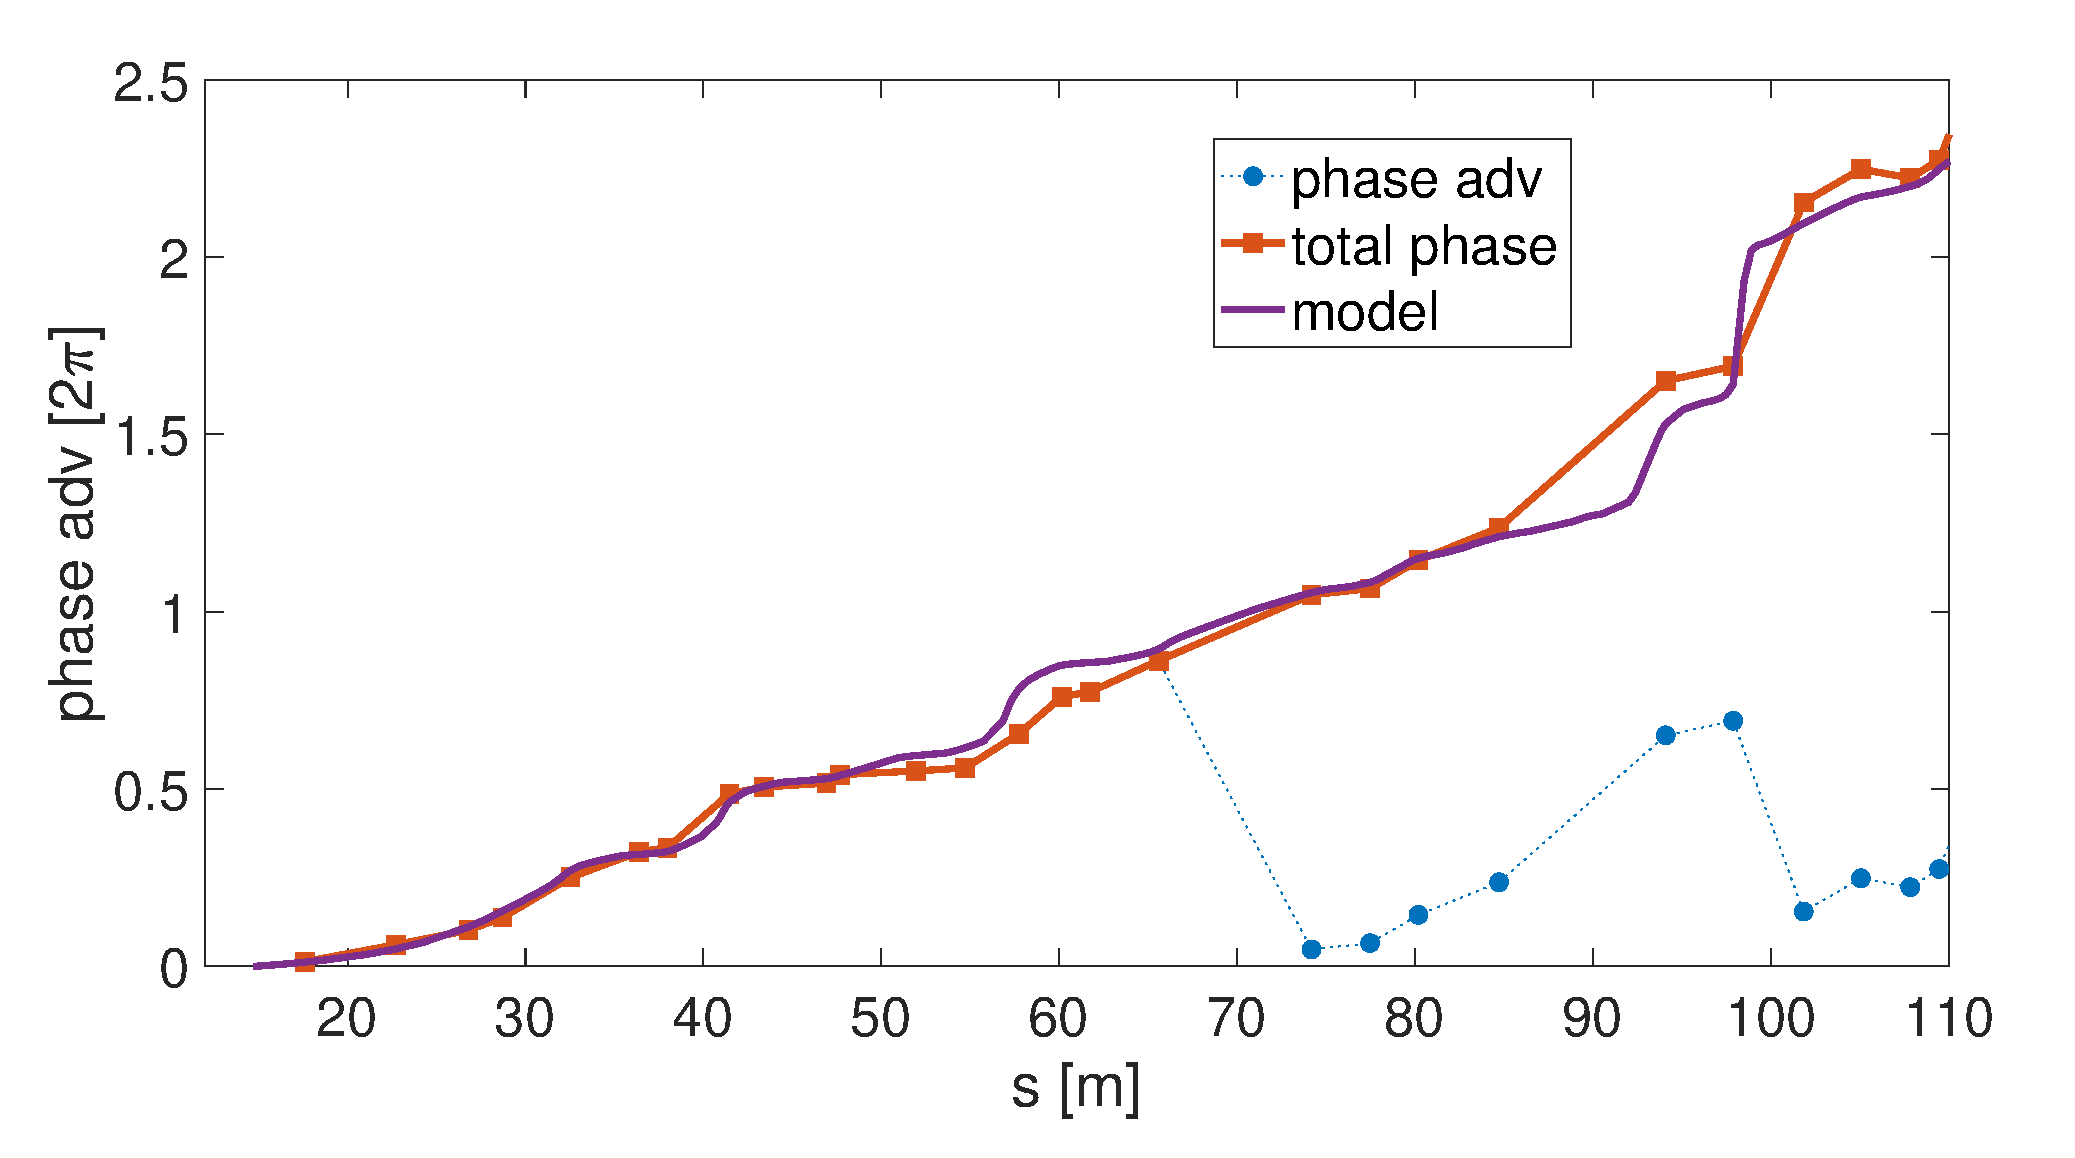
\includegraphics[width=0.49\columnwidth]{PhSPphase.eps}
    \label{fig:PhSPphase}} 
  \subfloat[]   %On the plot 15 Dec 2016 18:56
   {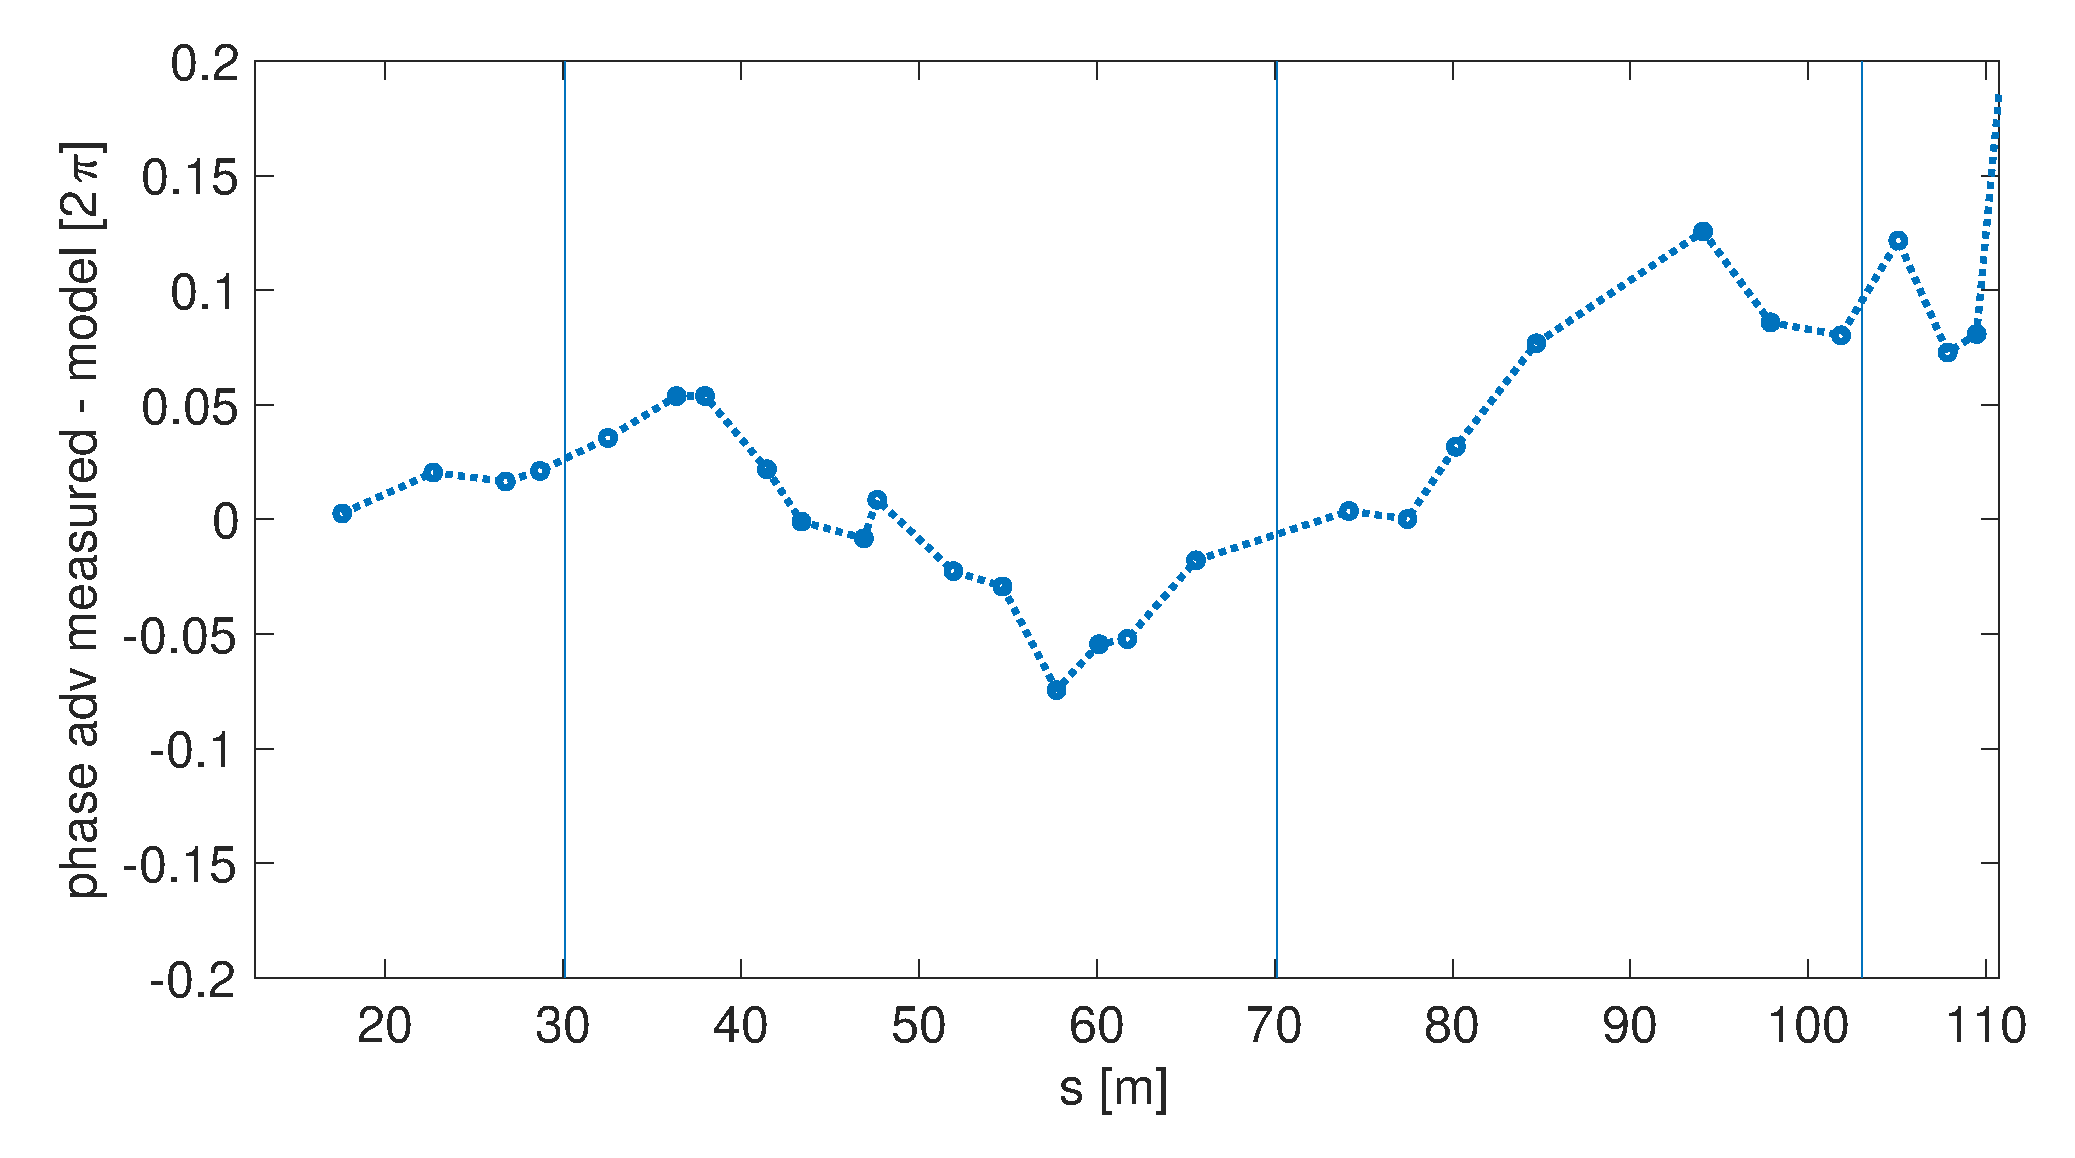
\includegraphics[width=0.49\columnwidth]{PhSPphase_diff.eps}
    \label{fig:PhSPphase_diff}}
 \caption{\protect\subref{fig:PhSPphase} Example of measured vertical phase advance and 
          \protect\subref{fig:PhSPphase_diff} its difference to the model.
          Vertical bars mark begining and end of the DL plus end of the TL1. }
 \label{fig:PhSpPhaseMeas}
\end{figure}


From phase differences between consequtive BPMs it was straight forward to obtain
the evolution of the phase advance along the machine, which was compared to the model
and eventually used for optics correction in conjunction with measured dispersion.
Figure~\ref{fig:PhSpPhaseMeas} presents an example measurement of CT line, DL and TL1
showing phase beating originating from the DL.

\textbeta -function was reconstructed using the 3-BPM method~\cite{bib:3BPMmethod}
\begin{equation}
\beta_{n} = \beta_{n~model}\frac{cot(\phi_{n-1}) + cot(\phi_{n+1}) }{cot(\phi_{n-1~model}) + cot(\phi_{n+1~model})}
\end{equation}
where $\phi_{n-1}$ is phase advance from the previous BPM and $\phi_{n+1}$ is to the following one.
This method assumes that the model transfer matrix between 2 consequtive BPMs is correct.
On the other hand, it not sensitive to BPM calibration errors.

The transfer matrix elements $R_{11}$ and $R_{12}$ between the location where the ellipse was painted
and given BPM were obtained by fitting function 
\begin{equation}
X_i = R_{11}X_{i0} + R_{12}*XP_{i0},
\label{eq:tm1}
\end{equation}
where $X_{i0}$ and $XP_{i0}$ are the painted coordinates defined by Equation~\ref{eq302_ellipseEq}.
Using Equation~\ref{eq:tm1} and the model values of the transfer matrix between consecutive
BPMs the momentum variable was reconstructed
\begin{equation}
XP_{n} = (X_{n+1} - X_{n})\frac{R_{11~model}}{R_{12~model}}.
\end{equation}
The reslting points were fitted with 
\begin{equation}
XP_i = R_{21}X_{i0} + R_{22}*XP_{i0},
\label{eq:tm2}
\end{equation}
allowing to find $R_{21}$ and $R_{22}$. Figure~\ref{fig:PhSpTM} illustrates an example measurement.

\begin{figure}[!h]
 \begin{center}
   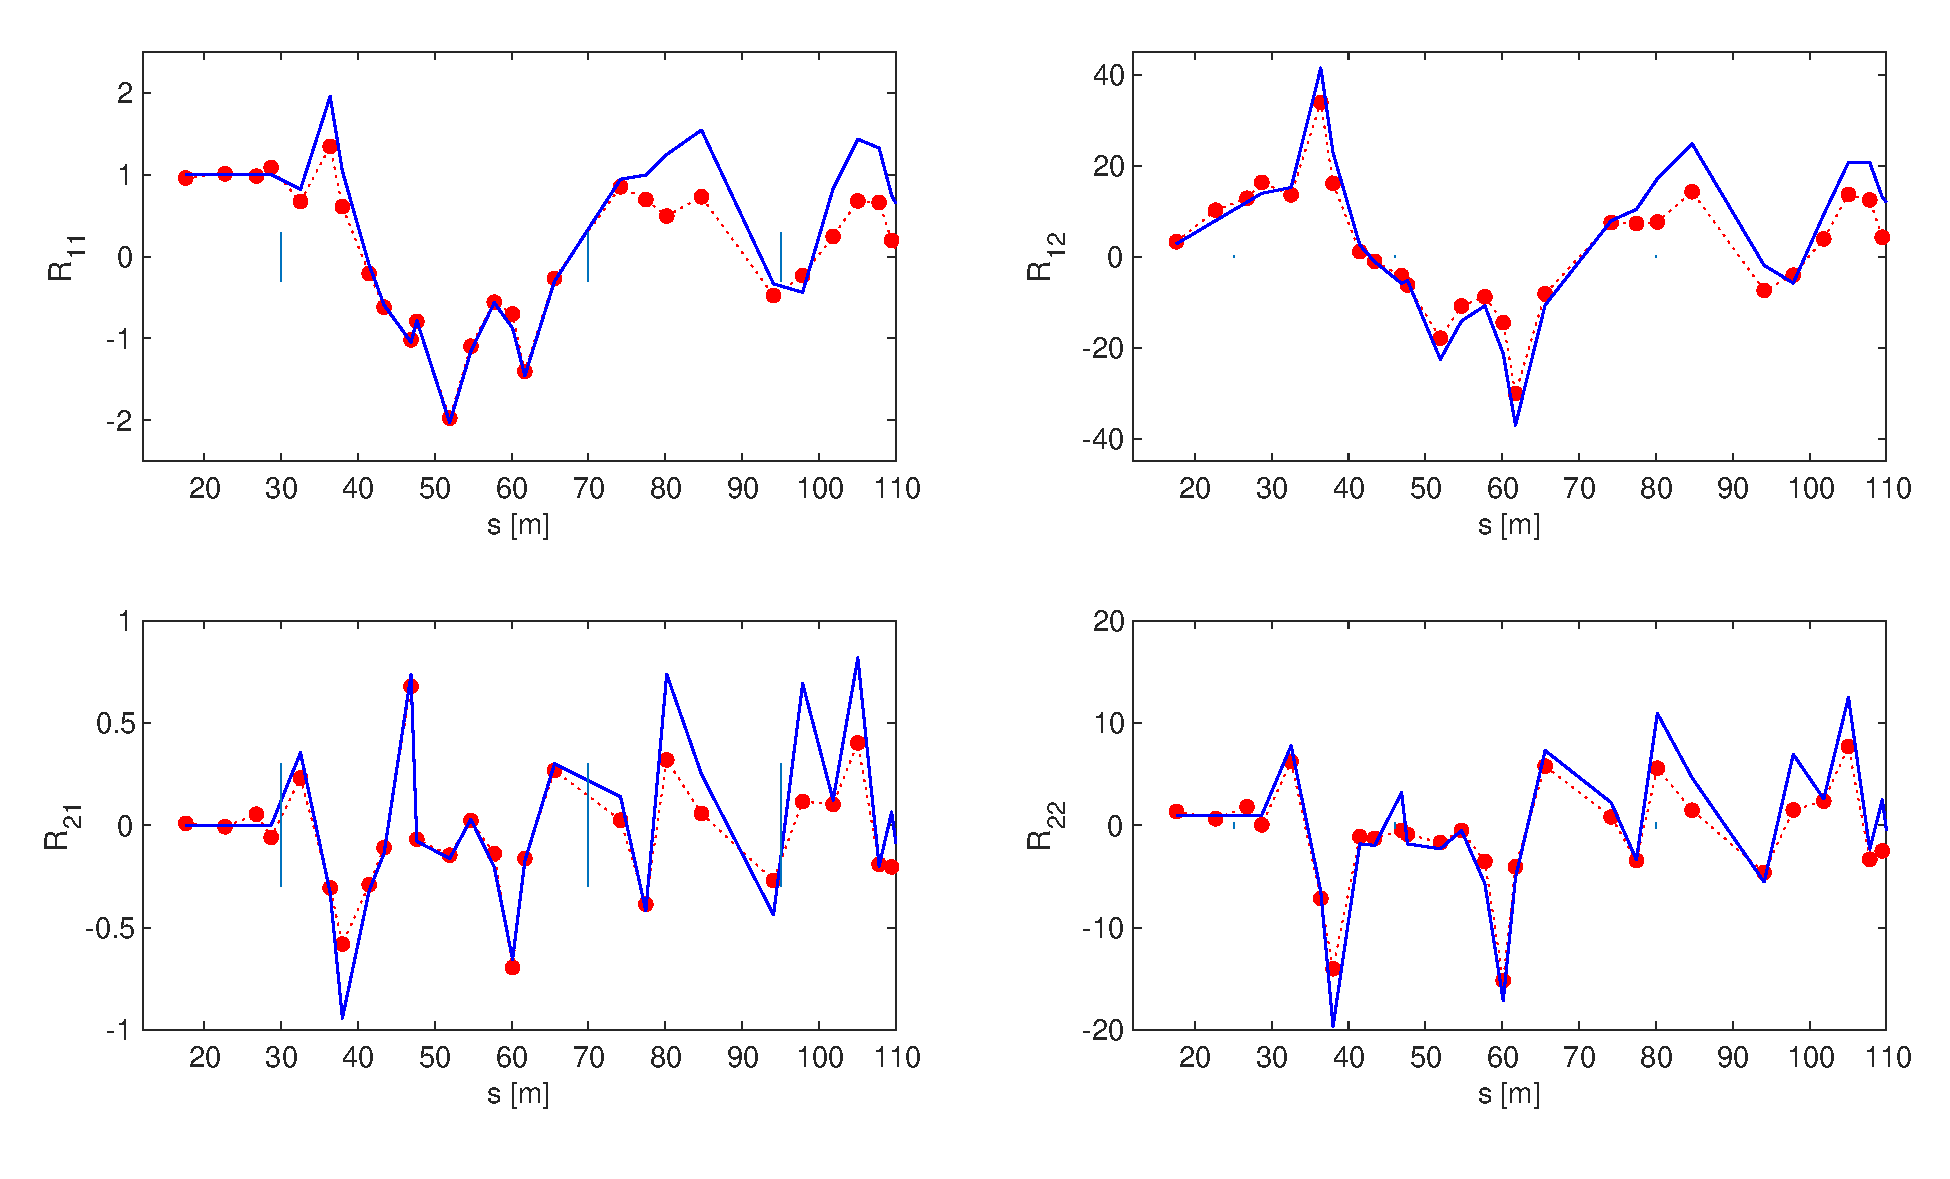
\includegraphics[width=0.99\columnwidth]{PhSPtm.eps} 
 \end{center}
 \caption{Example of measured vertical transfer matrix in 
          the CT, the DL and the TL1 illustrating an optics error.}
 \label{fig:PhSpTM}
\end{figure}


It was instructive to compare the obtained $X,XP$ with the model ellipse.
Ellipse equation was fitted yielding all Twiss parameters. 
Figure~\ref{fig:PhSpBeta} shows example of measured \textbeta -function 
using the described three methods in the CT, the DL and the TL1.

\begin{figure}[!h]
 \begin{center}
   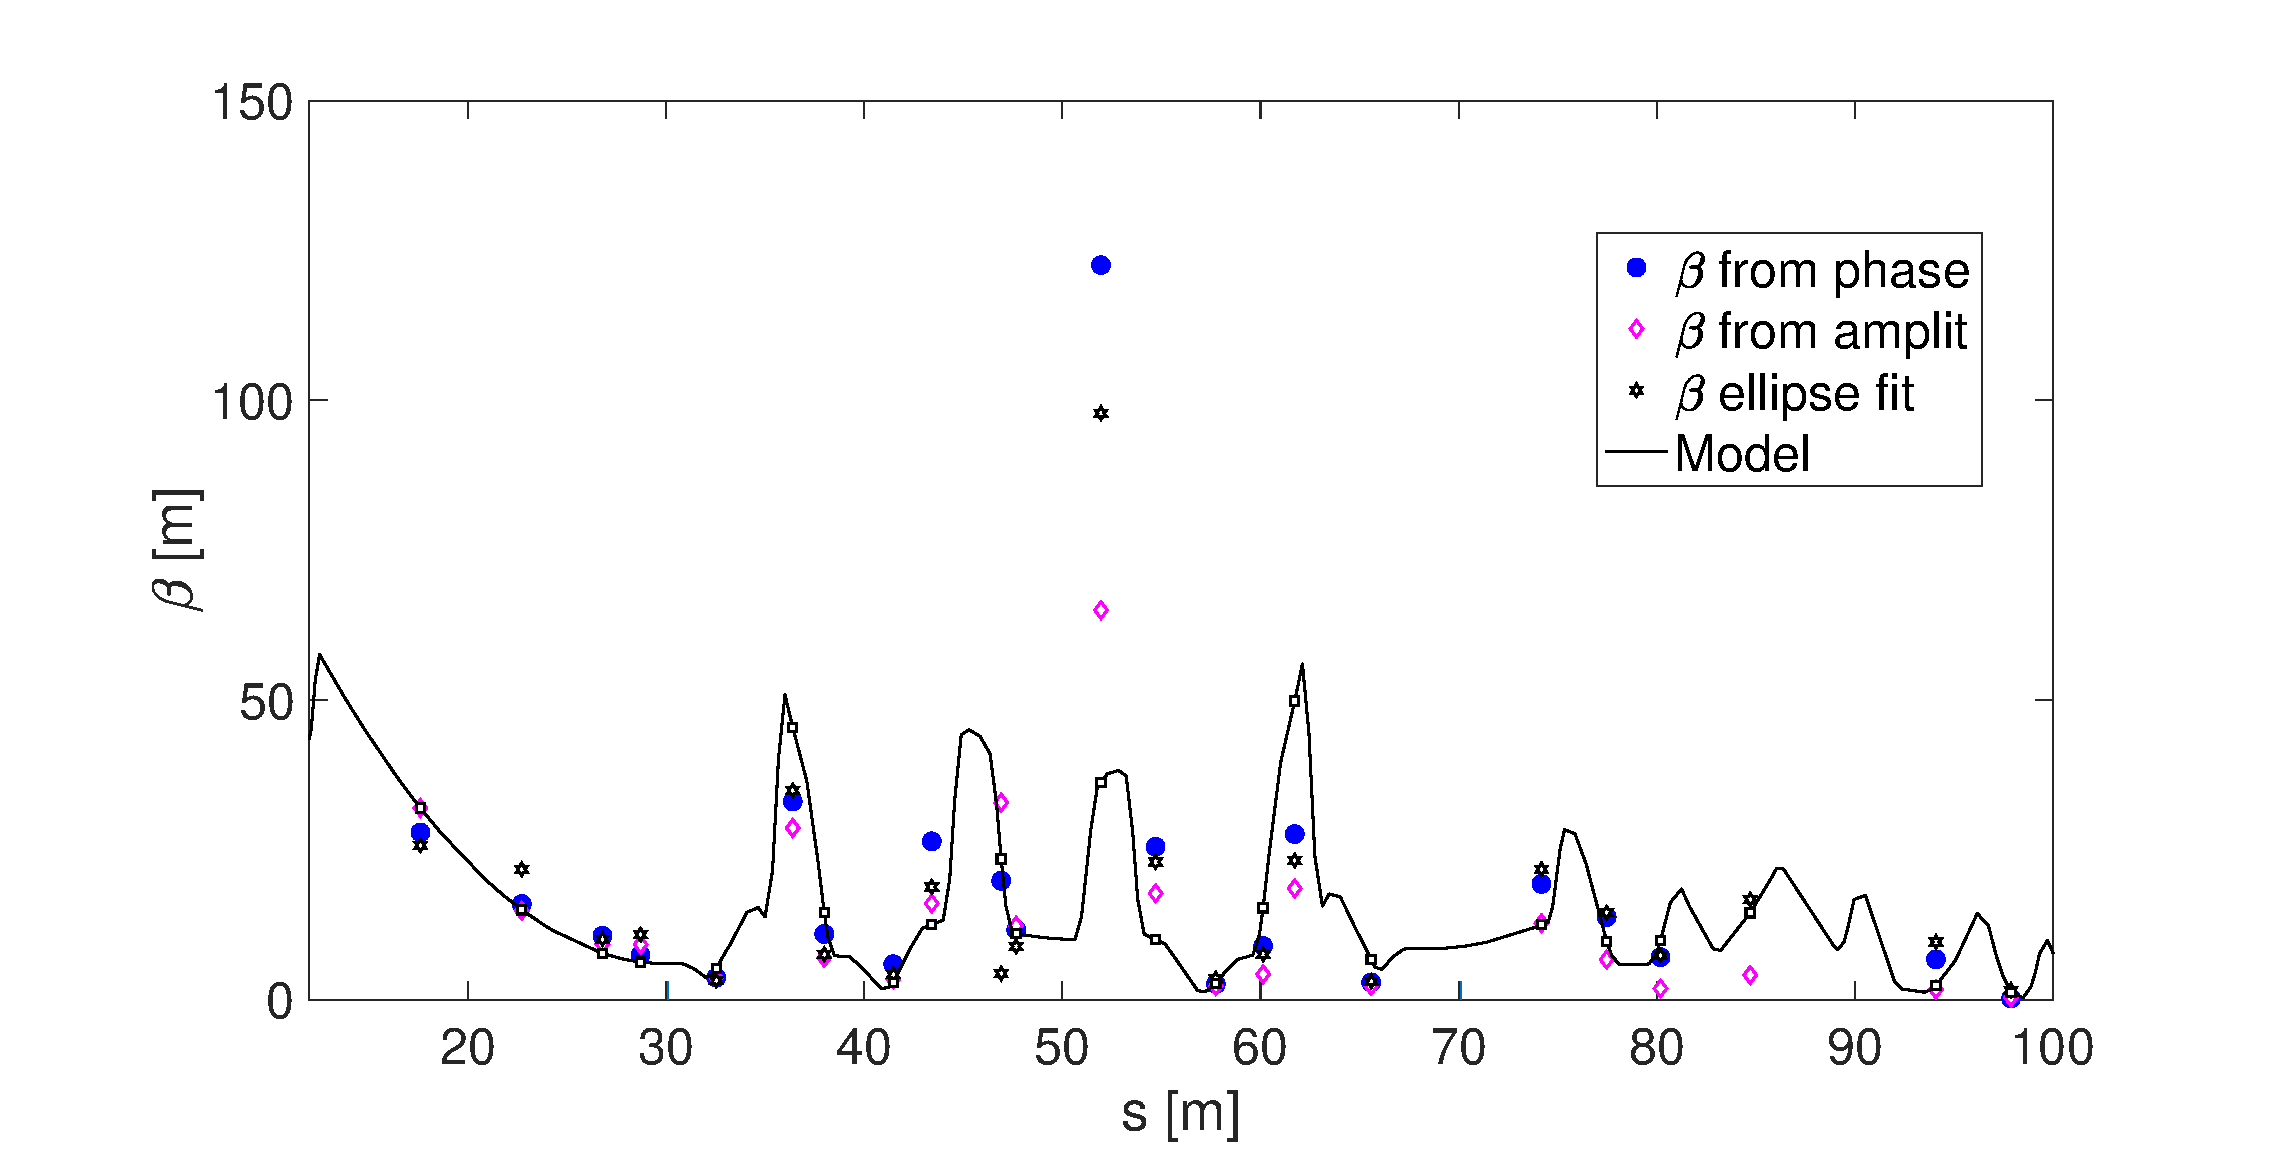
\includegraphics[width=0.75\columnwidth]{PhSPbeta.eps} 
 \end{center}
 \caption{Example of measured vertical \textbeta -function in the CT, the DL and the TL1.}
 \label{fig:PhSpBeta}
\end{figure}




 
